%%% Preamble
  \documentclass[11pt]{beamer}
  \usetheme{Boadilla}
  \useoutertheme{split}
  \useinnertheme{circles}
  \usepackage{fourier}
  \usefonttheme{structurebold}
  \usepackage{array}
  \usepackage[english]{babel}
  \usepackage{amsmath,amssymb}
  \usepackage[latin1]{inputenc}
  \usepackage{setspace}

  \usepackage{array}
  \usepackage{threeparttable}
  \usepackage{colortbl}
  \usepackage{multirow}
  \usepackage{amsthm}
  \usepackage{float,graphicx,color}
  \newtheorem*{thm}{Theorem}
  \theoremstyle{definition}
  \newtheorem*{defn}{Definition}
  \newcommand\boldline{\arrayrulewidth{1pt}\hline}
  \newcommand\ve{\varepsilon}
  \providecommand{\norm}[1]{\lVert#1\rVert}

  \setbeamercovered{dynamic}

  \title[Risky Time Series]{Risk Analysis using \\ARIMA and (G)ARCH Models}
  \author[Lyon]{\textbf{Spencer Lyon}}
  \date{\today}


\begin{document}

\frame{\titlepage}

\section{Intro}

\subsection{Class Exercise}

  \setstretch{1.75}
  \begin{frame}
    \frametitle{Risk Aversion Example}
    \begin{itemize}[<+->]
      \item Everyone gets to "invest" in one of two assets:
      \begin{enumerate}
        \item A guaranteed \$51,209
        \item A 50/50 chance of getting either \$50,000 or \$100,000.
      \end{enumerate}
      \item Raise hands and vote
    \end{itemize}
  \end{frame}

\subsection{The Equity Premium Puzzle (EPP)}

  \setstretch{1.2}
  \begin{frame}
    \frametitle{EPP History}
    \begin{itemize}[<+->]
      \item Seminal 1985 paper titled \textit{The Equity Premium: A Puzzle} by Mehra and Prescott
      \item Discovered odd relationship between demand for risky and risk free assets
      \item Can be summarized with 1 of 2 questions:
      \begin{enumerate}
        \item Why is demand for risk free government bonds so high when returns on those assets are so low?
        \item Why is demand for stocks, and hence stock prices, so low despite the relatively high expected returns?
      \end{enumerate}
    \end{itemize}
  \end{frame}

  \begin{frame}[t]\frametitle{Possible Explanations}
    \begin{itemize}[<+->]
      \item Some say it doesn't exist. The data says it does!
      \item Risk Aversion:
      \begin{itemize}
        \item Stocks are risky assets so people are less willing to invest in them.
        \item Very Incomplete $\rightarrow$ In 1991 Mankiw showed that investors would be indifferent between our assets from the beginning using standard risk aversion coefficients.
      \end{itemize}
      \item Market Failures: things like transaction costs or liquidity constraints
      \item Volatility arguments: Risky assets are much more volatile - people don't like that.
      \item Tax policy
    \end{itemize}
  \end{frame}

\section{Data}

  \begin{frame} \frametitle{My Data}
    \begin{itemize}
      \item Risky Assets:
        \begin{itemize}
           \item Prices for SP500 (\^{}GSPC)
           \item Value of VIX (\^{}VIX)
         \end{itemize}
      \item Risk Free Assets:
        \begin{itemize}
          \item 3-Month US T-bill (DGS3MO)
          \item 10-Year US T-bill (DGS10)
        \end{itemize}
        \item Frequency for all data is Business Day
        \item Collected from 1-1-1990 to 4-8-2013
    \end{itemize}
  \end{frame}

  \begin{frame}[t]\frametitle{Plot Data}

    \begin{figure}[ht]
          \centering
          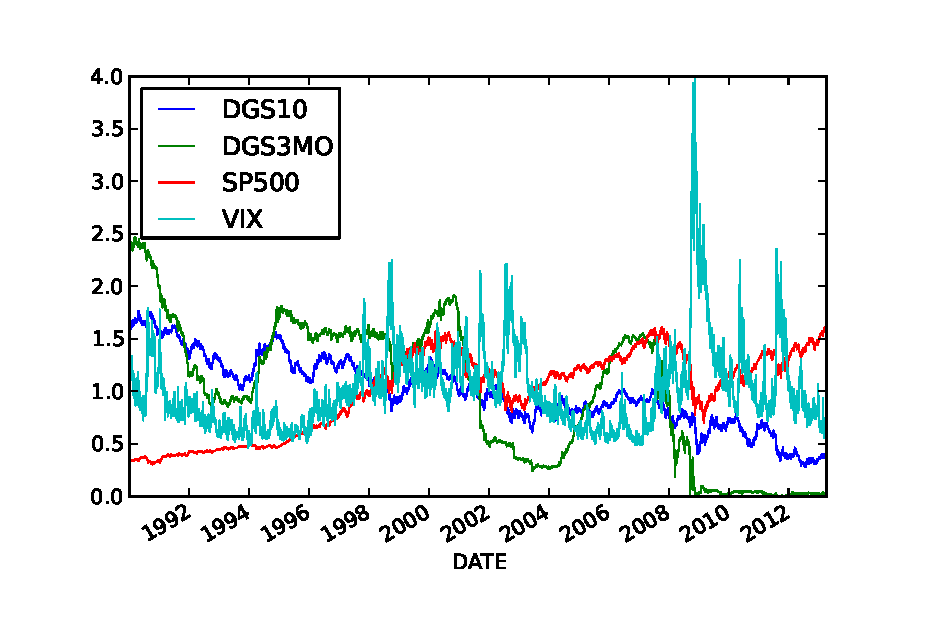
\includegraphics[width=4in]{.././Figures/all_data.eps}
          \caption{\small Plot of the data used in this paper. Note that because the units are different and the value of the S\&P 500 is much larger than the percents on the T-bill data sets, I have divided each data set by its mean before plotting.}
          \label{fig:alldata}
      \end{figure}

  \end{frame}

\section{My Work}

  \subsection{The Plan}
  \begin{frame} \frametitle{Plans}
    \begin{itemize}[<+->]
      \item My Question: Will standard, modern time series techniques forecast data in line with the EPP or against it?
      \item I will use ARIMA, GARCH, and ARCH models to generate forecasts for the data
      \item I will then see what the implied equity premium is on my forecasted data
    \end{itemize}
  \end{frame}

  \subsection{ARIMA}
  \begin{frame}\frametitle{Setting up ARIMA}

  \begin{itemize}[<+->]
    \item Need to identify p, q, d for arima.
    \item For finding p and q see Figure on next slide (p=1, q=0 for all)
    \item To find d I saw how many times I needed to difference the data to get stationary. See table in 2 slides(d=1 for all).
  \end{itemize}

  \end{frame}

  \begin{frame}\frametitle{PAC and AC}

    \begin{figure}[!h]
          \centering
          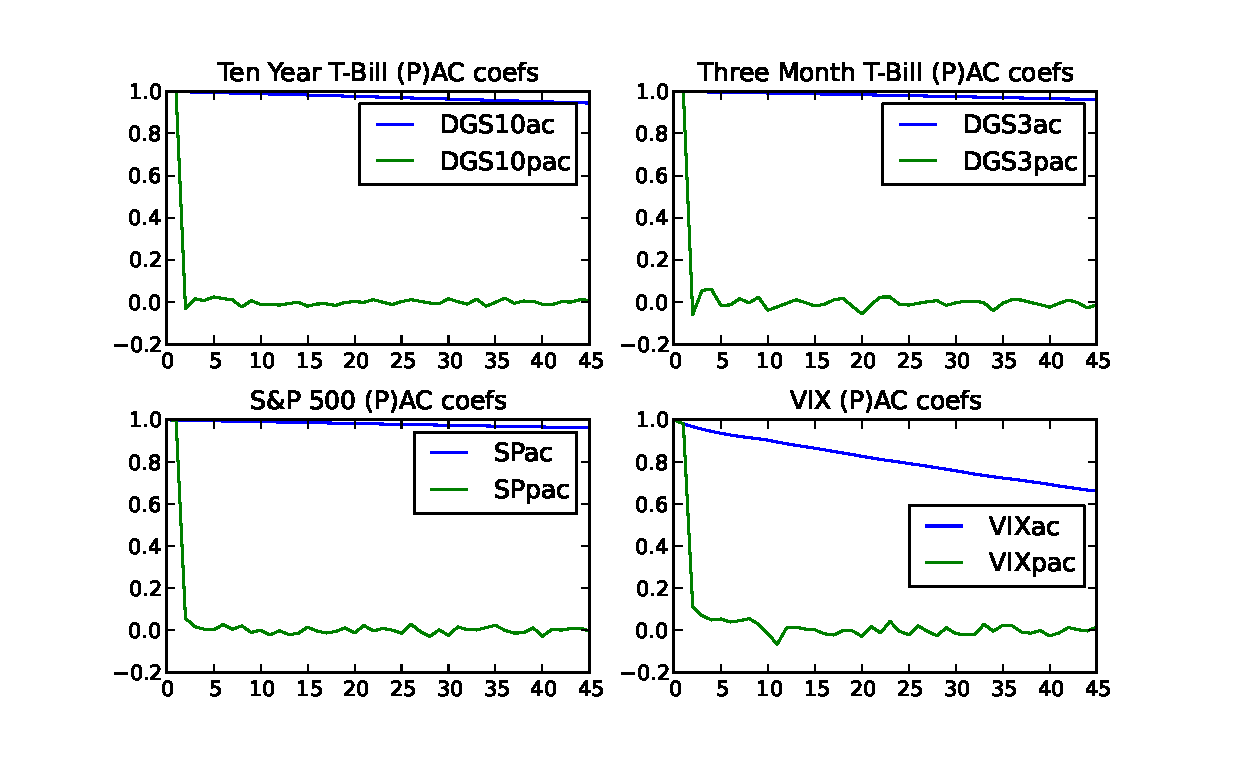
\includegraphics[width=4in]{../Figures/all_corrs.eps}
          % \caption{\small Autocorrelation and partial autocorrelation coefficients for each data set. Used to find the parameters $q$ and $p$ in an ARIMA model.}
          \label{fig:correlations}
      \end{figure}

  \end{frame}

  \begin{frame}\frametitle{Moments for Differences}

    \begin{table}
      \label{tab:differences}
      \setstretch{1.25}
      \scalebox{0.75}{
      \begin{tabular}{|l|c|cc||l|c|cc|}
        \hline
         \rowcolor{blue!40} DataSet & Lags &   Mean &     Variance & DataSet & Lags &   Mean &     Variance \\
        \hline
        \hline
         \rowcolor{blue!7} DGS10  & 1    & -0.001425545 &  0.003990852 & SP500  & 1    &   0.03449455 &  224.2908 \\
         \rowcolor{blue!23} {} &     2    & -0.002824705 &  0.007977331 & {} &     2    &   0.08398426 &  406.3557 \\
         \rowcolor{blue!7} {} &     3    &  -0.00424894 &   0.01156277 & {} &      3    &    0.1329679 &   574.528 \\
         \rowcolor{blue!23} {} &     4    & -0.005655862 &   0.01518609 & {} &     4    &    0.1779158 &  748.1064 \\
         \rowcolor{blue!7} DGS3MO &  1    & -0.001637409 &  0.003366346 & VIX    & 1    & -0.003483656 &   3.13206 \\
         \rowcolor{blue!23} {} &     2    & -0.003254617 &  0.007774232 & {} &     2    & -0.007680896 &  5.355797 \\
         \rowcolor{blue!7} {} &     3    &  -0.00488189 &   0.01147704 & {} &     3    &  -0.01181405 &  7.261939 \\
         \rowcolor{blue!23} {} &     4    & -0.006498031 &   0.01407682 & {} &     4    &  -0.01544986 &  9.018458 \\
        \hline
      \end{tabular}}
      \setstretch{1.75}
    \end{table}
  \end{frame}

    \subsection{(G)ARCH}

    \begin{frame}\frametitle{GARCH}
        I still need to do this
    \end{frame}


\end{document}
